\documentclass{article} % For LaTeX2e
\usepackage{style-file,times}
\usepackage{hyperref}
\usepackage{url}
\usepackage{graphicx}
\usepackage[numbib,notlof,notlot,nottoc]{tocbibind}

\title{Project Proposal: Creating Playlist Names using Tracklist Information}

\author{
    Team: Sofia Samaniego de la Fuente (SUID: sofiasf) \\
    \texttt{\footnotesize sofiasf@stanford.edu} \\
}

\newcommand{\fix}{\marginpar{FIX}}
\newcommand{\new}{\marginpar{NEW}}

\nipsfinalcopy % Uncomment for camera-ready version

\begin{document}

\maketitle

%\begin{abstract}
%\end{abstract}

\section{Problem Description}
\label{description}
The goal is to implement a model that comes up with a name for a playlist given information about its tracklist. 
In particular, we will attempt to construct a network that builds an internal representation of the names of the tracks included in the playlist and then uses natural language generation techniques to come up with a title that could be close to one a human might devise. 

\section{Data}
\label{data}
Spotify recently released the \emph{Million Playlist Dataset}, official website hosted at \href{https://recsys-challenge.spotify.com}{https://recsys-challenge.spotify.com}, as part of its 2018 RecSys Challenge.
It comprises a set of $1,000,000$ playlist that have been created by Spotify users along with a variety of features, including playlist name, description, timestamp when the playlist was last updated, and an array of information about each track in the playlist (track name, artist, album name, duration, position in the playlist).
Additionally, Spotify provides a \textsf{python} script that computes the following statistics for the dataset:

\begin{table}[h!]
\caption{Statistics for the \emph{Million Playlist Dataset}}
\centering
 \begin{tabular}{|lr|} 
 \hline
 	Number of playlists & 1000000 \\
	Number of tracks & 66346428 \\
	Number of unique tracks & 2262292 \\
	Number of unique albums & 734684 \\
	Number of unique artists & 295860 \\
	Number of unique titles & 92944 \\
	Number of playlists with descriptions & 18760 \\
	Number of unique normalized titles & 17381 \\
	Avg playlist length & 66.346428 \\     
 \hline
 \end{tabular}
\end{table}


\begin{table}[h!]
\caption{Top playlist names, artists, and songs (with counts)}
\centering
  \begin{tabular}{|c|c|c|} 
  	\hline 
  	Playlist Title & Track & Artist \\
  	\hline
  	Country  & HUMBLE. by Kendrick Lamar  & Drake  \\ 
  	Chill  & One Dance by Drake  & Kanye West  \\
  	Rap  & Broccoli (feat. Lil Yachty) by DRAM  & Kendrick Lamar  \\
  	Workout  & Closer by The Chainsmokers  & Rihanna  \\
  	Oldies  & Congratulations by Post Malone  & The Weeknd  \\
  	Christmas  & Caroline by Aminé  & Eminem  \\
  	Rock  & iSpy (feat. Lil Yachty) by KYLE  & Ed Sheeran  \\
  	Party  & Bad and Boujee (feat. Lil Uzi Vert) by Migos  & Future  \\
  	Throwback  & Location by Khalid  & Justin Bieber  \\
  	Jams  & XO TOUR Llif3 by Lil Uzi Vert  & J. Cole \\
  	\hline
 \end{tabular}
\end{table}

\begin{figure}
  \centering
  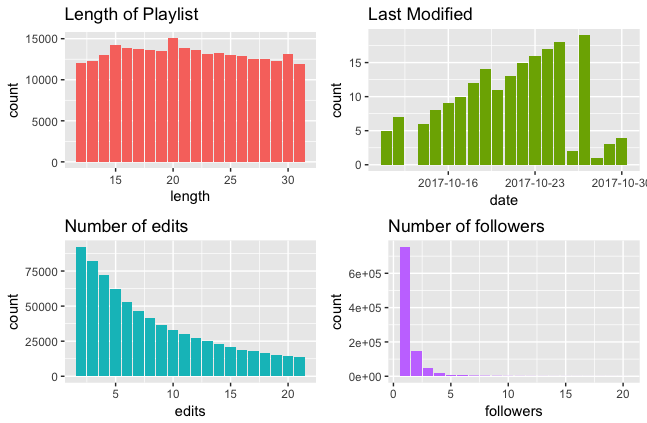
\includegraphics[width = 0.8\textwidth]{histograms.png}
  \caption{Histograms for selection of variables}
  \label{fig:boat1}
\end{figure}



\section{Methodology}
\label{methods}
Coming up with a playlist name is somehow related to the task of creating a condensed representation of an input text, namely the names of the songs contained in it, the artists that perform them, and their genres.
Therefore, we could try to use automatic summarization techniques for this purpose. In particular, we could achieve this in two ways: through extractive summarization, that is, by choosing a subset of words in the original input that capture the gist of the playlist, or though abstractive summarization, that is, by generating a new title that conveys the relevant information, aspects of which may not appear in the input text.  
One way to modify such methods would be to somehow introduce the numerical features we have available (such as duration of the platlist, number of unique artists, time created) as additional input to our neural network, as this might help the network come up with better names for the playlists.

\section{Related Work}
\label{work}
To inform our understanding of automatic summarization and the mehology to tackle this problems, we propose the following references:
\begin{itemize}
	\item \textbf{A neural attention model for abstractive sentence summarization}\cite{rush2015neural}, by Rush, Alexander M and Chopra, Sumit and Weston, Jason.
	\item \textbf{Abstactive text summarization using sequence-to-sequence RNNs and beyond}\cite{nallapati2016abstractive}, by Nallapati, Ramesh, and Zhou.
	\item \textbf{Opinosis: a graph-based approach to abstractive summarization of highly redundant opinions}\cite{ganesan2010opinosis}, by Ganesa, Kavita and Zai. 
\end{itemize}

Meanwhile, for a better understanding of generative language techniques, we propose the following references: 
\begin{itemize}
    \item \textbf{Generating text with recurrent neural networks}\cite{sutskever2011generating} by Sutskever, Ilya and Martens, James and Hinton, Geoffrey E.	
    \item \textbf{System and method for natural language generation}\cite{bangalore2007system} by Bangalore, Srinivas and Rambow, Owen Christopher. 
    \item \textbf{Generating sentences from semantic vector space representations}\cite{iyyer2014generating} by Iyyer, Mohit and Boyd-Graber, Jordan and Daum{\'e} III, Hal. 
\end{itemize}

Other good sources of inspiration could be the following blogposts:
\begin{itemize}
	\item \href{https://medium.com/deep-writing}{Deep Writing (Medium)}
	\item \href{https://blog.paperspace.com/recurrent-neural-networks-part-1-2/}{Recurrent Neural Networkds (Paperspace)}
	\item \href{https://ehudreiter.com/2016/12/12/nlg-and-ml/}{Natural Language Generation and Machine Learning (Ehud Reiter's Blog)}


\section{Evaluation Plan}
Deciding whether a playlist name is `good" is a highly subjective task and best determined by human judgement, so coming up with an automatic evaluation metric could be particularly difficult.
One possibility would be to to calculate the n-gram overlap between automatically generated playlist titles and previous titles devised by humans, as proposed in NIST's annual Document Understanding Conferences (this metric is known as ROUGE: Recall-Oriented Understudy for Gisting Evaluation).
However, this could lead to bad scores for creative titles that no humans have come up with before.


\nocite{namas}
\nocite{rnnlg}
\bibliographystyle{plain}
\bibliography{references}

\end{document}
